\chapter{Generating English Synthetic Documents with Clinical Keywords: A Privacy-Sensitive Methodology}

Electronic Health Records (EHR) store valuable patient-staff interaction data. These notes, often unstructured to save healthcare personnel time, can be challenging to analyze manually. Proprietary online LLMs have demonstrated impressive results in analyzing EHR notes. However, Clinical NLP faces unique challenges due to the sensitive and specialized nature of the data. Sending patient information via external APIs poses privacy risks, and hospitals require customized NLP systems to align with their practices. Developing customized LLMs using specific training datasets is crucial to address these challenges. 
We propose generating synthetic training data using keywords extracted without confidential information. Furthermore, we introduce a reward mechanism that iteratively refines the quality of synthetic documents. This involves scoring synthetic candidates against real clinical reports using a semantic textual similarity score and performing an alignment step to align the model with its best-scored utterances.

\section{Introduction}

Electronic Health Records (EHR) contain patient and healthcare staff interactions. Professionals record their impressions, observations, and various medical procedures performed. Despite the computerization of clinical documents, notes remain fairly expressive and in a free format to save time for healthcare personnel and allow for the description of unusual situations \citep{rosenbloomDataClinicalNotes2011,wuSurveyClinicalNatural2022}. These notes can be handy for medical professionals, but analyzing them manually is daunting. Natural Language Processing (NLP) techniques come here, as they speed up the decision processes \cite{zhouDataSifterTextPartiallySynthetic2022,wuSurveyClinicalNatural2022}.

In recent years, Proprietary Online Large Language Models (LLMs) such as ChatGPT have shown impressive results using zero or few-shot techniques in analyzing these notes \cite{agrawal_large_2022, meoniLargeLanguageModels2023, hu_improving_2024}.

However, clinical NLP faces challenges that arise from the sensitive, confidential, and specialized nature of its data—sending such information through an external API risks patient privacy. Hospitals must maintain control over their NLP systems due to their unique practices and environments. Creating customized LLMs is an important issue.

A specific training dataset is required to develop such a model with clinical skills. Accessing real clinical data to constitute this dataset remains very complex and requires anonymization, which is time-consuming and expensive. 

Another option is to generate synthetic clinical notes that resemble real data and do not contain any patient identifiers \cite{melamud_towards_2019, ive_generation_2020}. This approach reduces human intervention and is more compliant with regulation laws.

\section{Contributions}

This work introduces a novel method for generating synthetic documents, enforcing privacy preservation by design, only using sparsely pseudo-anonymised data. Our key contributions include:

\paragraph{Privacy-conscious Synthetic Document Generation:} 
    We propose a methodology that utilizes a small amount of manually anonymized data to generate synthetic documents. These documents are then used to supervise fine-tuned generators, as illustrated in Figure \ref{fig:synth_workflow}.

\paragraph{Incorporating Clinical Keywords:} We enhance synthetic document generation by enriching prompts with privacy-safe keywords as illustrated in Figure~\ref{fig:synth_prompt}. Using QuickUMLS \citep{soldaini_quickumls_nodate}, we generate candidate documents based on keywords extracted from real Clinical reports (\crt). The keywords guide the model to produce text that closely aligns with specified content and style criteria.

\paragraph{Reward Mechanism:} We introduce an iterative refinement process for enhancing the quality of the synthetic documents generated by the seeded model. This method involves two main key steps: 
    \begin{itemize}
        \item Scoring the synthetic candidates through comparison with private or real \crt using an \score evaluator model in the private side returning only scores to the public side; % this model is the only one accessing private data
        \item Aligning the model with its best utterances using Direct Preference Optimization (DPO) \citep{rafailov_direct_2023}.
    \end{itemize}

\begin{figure}
    \centering
    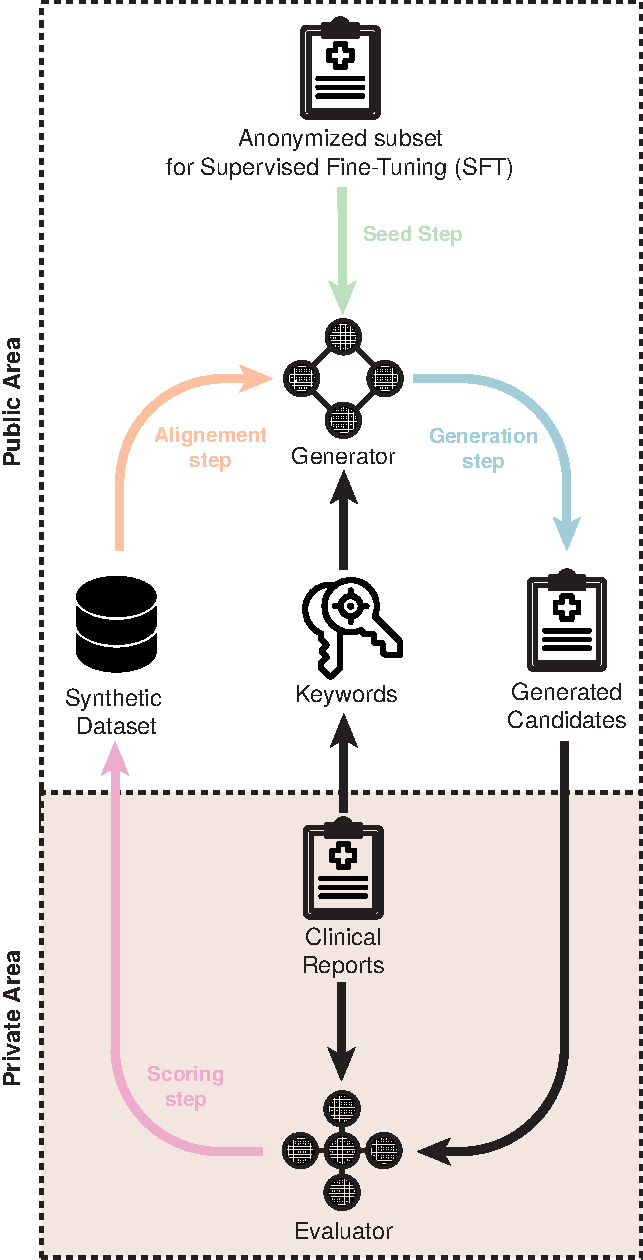
\includegraphics[width=0.9\textwidth]{figures/synthetic_generation/workflow.pdf}
    \caption{Our workflow is delimited by the private and public areas. Only the score is returned to the public area.}
    \label{fig:synth_workflow}
\end{figure}

\section{Related Works}

\paragraph{Synthetic Data Generation:}
Recent works tend to generate synthetic data with privacy concerns \cite{liTwoDirectionsClinical2023, hiebelCanSyntheticText2023, xie_differentially_2024, li_synthetic_2024}. For instance, \cite{kweon_publicly_2023} proposes to train LLMs for different purposes using synthetic clinical data generated by online LLMs. This way, \cite{xie_differentially_2024} has developed AUG-PE, a high-quality differential privacy synthetic text generation method leveraging API access. Furthermore, the work by \cite{li_synthetic_2024} introduces Generalized Instruction Tuning (GLAN). Unlike previous approaches that rely on seed or existing datasets, GLAN uses a pre-curated taxonomy of human knowledge and capabilities as input to generate instructions across all disciplines. 

\paragraph{Self-Rewarding:}
Reinforced Self-Training is an offline RL algorithm proposed by \cite{gulcehre_reinforced_2023} for self-align LLMs generating a dataset from the initial LLM policy and using it to improve the policy via offline RL. Instruction back translation, proposed by \cite{li_self-alignment_2023}, is a scalable method that automatically labels human-written text with corresponding instructions by finetuning a language model on a small seed dataset and a web corpus to generate and selecting high-quality examples for further finetuning. \cite{yuan_self-rewarding_2024-1} use the trained LLM to provide rewards via LLM-as-a-Judge prompting, leading to improvements in both instruction following and reward provision.

Our method differs from the methods described above in these differences : 
\begin{itemize}
    \item only the score is accessible to the learner, preserving the privacy of real EHR.
    \item only public medical keywords extracted from EHRs are used to generate synthetic data
    \item the \score evaluator can be easily hosted in a clinical environment and the generator LLM may be shared with external actors.
\end{itemize}

\section{\score as Evaluation Metrics}

To evaluate the quality of the responses generated by an instruction-tuned LLM, we adopt \score, a metric based on semantic textual similarity (STS). However, we add two differences with SEMSCORE \citep{aynetdinov2024semscore}:
\begin{enumerate}
\item we embed generated document and ground truth using \space\verb|all-distilroberta-v1|, fine-tuned on synthetic documents as described in section \ref{sec:synth_score}
\item We compute the similarity between model and target responses through the cosine similarity of their embeddings.
\end{enumerate}
The interval $[-1, 1]$ represents the value where $1$ indicates similarity and $-1$, semantic opposition between a pair of two sequences. Based on textual similarity, \textit{\score exhibits the strongest correlation to human evaluation results, even outperforming LLM-based metrics, while not requiring special access or incurring additional cost}. We can use this metric in a real-world scenario where the model (\me) must be hosted in the clinical building to measure STS between private clinical and synthetically generated reports.    

\section{Reward Training}
\label{sec:synth_method}

\begin{algorithm}
\caption{Reward Training Algorithm}
\label{alg:synth_method}
\SetKwInOut{Input}{Input~}
\SetKwInOut{Output}{Output~}
\SetKwFor{For}{for}{do}{endfor}
\SetKwIF{If}{ElseIf}{Else}{if}{then}{else if}{else}{endif}
\SetKwFunction{Sample}{Sample}
\SetKwFunction{Anon}{Anonymize}
\SetKwFunction{Extract}{ExtractKeywords}
\SetKwFunction{ContrastiveTrain}{ContrastiveTrain}
\SetAlgoLined
\DontPrintSemicolon
\Input{\dtr = train dataset; \rsft = sft ratio; \rgen = gen ratio; \mg = generative model; \me = evaluator model; $p$ = percentile filter value; $N$ = number of candidates to generate;}
\Output{\mg}
\ktr $\gets$ \Extract{\dtr}\;
\dsft,\space\ksft $\gets$ \Anon{\Sample{\dtr, \ktr,\space\rsft}}\;
\dgen,\space\kgen $\gets$ \Sample(\dtr, \ktr,\space \rgen)\;
\textcolor{seedStep}{\tcp{\textbf{Seed Step}}}
\mg $\gets$ Supervised fine-tune \mg on pairs in (\ksft, \dsft)\;
\For{$step = 1$ \KwTo $steps$}{
    \textcolor{genStep}{\tcp{\textbf{Generation Step}}}
    $D^{*}_{gen} \gets$ generate new $N$ candidates with \mg per $k\in$ \kgen\;
    \colorbox[HTML]{F3E6E0}{\parbox{0.95\dimexpr\linewidth-2\fboxsep-2\fboxrule}{
   \textcolor{scoringStep}
    {\tcp{\textbf{Scoring Step}}}
    \If{$step = 1$}{
    \textcolor{scoringStep}
    {\tcp{\textbf{Building the evaluator model}}}
        \dcstar, \dc $\gets$ \Sample{$D^{*}_{gen}$, 
        $D_{gen}$,
        \space$ratio_{contr}$}\;
        %$D_{contr}$ $\gets$ %\Sample{$D_{gen}$,\space$rat%io_{contr}$}\;
        \me $\gets$ \ContrastiveTrain(\me,\space neg=$D^{*}_{constr}$,\space pos=$D_{constr}$)\;
    }
    $D_{score} \gets$ score $D^{*}_{gen}$ over $D_{gen}$ with \me over the candidates generated\;}}
    $D_{dpo} \gets$ for each data point in $D_{score}$, keep a pair of candidates, then filter pairs on percentile $p$\;
    \textcolor{alignStep}{\tcp{\textbf{Alignement Step}}}
    \mg $\gets$ DPO Alignment \mg on (\kgen, $D_{dpo}$)\;
}
\end{algorithm}

The task aims to generate synthetic CRs with prompts enriched with keywords (Figure \ref{fig:synth_prompt}) extracted on real CR as illustrated in Figure \ref{fig:synth_workflow}. As preprocessing, we collect in \ktr, keywords for each document in \dtr, keeping in mind that these keywords do not carry confidential information.

\subsection{Seed Step}
Keeping associated keywords in \ksft, we sample, with ratio \rsft, a very small subset of the training dataset \dtr to fine-tune, after deidentification, our initial generator model \mg.

\subsection{Generation Step}
For each data point in \kgen, \mg\ generates $N$ candidate documents collected in dataset \dgen.

\subsection{Scoring Step}
\label{sec:synth_score}
The scoring step consists of two steps:
\begin{enumerate}
    \item at the first generation step ($step = 1$), we initialize the evaluator model \me, fine-tuning it with a contrastive objective on \dcstar and \dc correspond to a split of \dgstar with the respective real documents from \dgen.
    
    \item With \me we score candidates from \dgstar over 
    \dgen, we select a pair of \textit{chosen} and \textit{rejected} items among $N$ candidates where the chosen (resp. rejected) one is the candidate with the maximum (resp. minimal) score. Finally, we keep the pair where the chosen candidate is above the percentile $p$ to obtain \ddpo.
\end{enumerate}

\subsection{Alignment Step}
We align and update \mg using DPO on \ddpo and pursue a new iteration as illustrated by Algorithm~\ref{alg:synth_method}. 

\section{Experiments}
\label{sec:synth_experiment}

\newtcolorbox{modelinput}{colback=blue!5!white,colframe=blue!75!black}
\begin{figure}
\centering
\begin{modelinput}
\verb|<s>[INST]|As a doctor, you must write an original 'History of Present Illness' (HPI) section for a discharge summary.
Your response should capture the essence of a patient's health journey and recent medical experiences while strictly using all the provided keywords, preserving the order.
You must adopt a medical telegraphic style, abbreviated, characterized by concise and direct language.
\\
\textbf{Keywords:} \textit{cirrhosis c, portal, esophageal varices, SBP, angioectasias, gout, liver, note, fractured, left wrist, hip, note, admissions, asymptomatic, range, PRBCs, angioectasias, estrogen, bleeding, hospital course, SBP, guaiac, stool, L wrist, L hip, consulted, L wrist, leg, said, surgical, pantoprazole, gtt, morphine, hip pain, PRBCs, transfer, sat, hip pain, esp, feeling, note, iron, stools, stools}\verb|[/INST]|
\end{modelinput}
\caption{Example of prompt with injected keywords}
\label{fig:synth_prompt}
\end{figure}    

\paragraph{Model:} we use \space\verb|Mistral-7B-Instruct-v0.1|\space\citep{jiangMistral7B2023}, a trade-off between performance and computational cost. We use \verb|QLoRA|\space\citep{dettmers_qlora_2023} reducing the memory footprint.

\paragraph{Dataset:}
Our dataset is derived from the \mimic database, applying a protocol to ensure its applicability to generate clinical narratives. The creation process includes pre-processing, keyword extraction and post-processing steps.
\begin{enumerate}
    \item \textit{pre-processing}: we extract from \mimic the clinical notes from the clinical event row. We select only the \textit{Discharge Summaries} from these clinical notes and parse them to retrieve the \textit{History of Patient Illness} section. we use them as data points for our \dtr. On average, the data points consist of a 248-word excerpt.
    \item \textit{keywords extraction}: We project UMLS concepts using QuickUMLS over \dtr. QuickUMLS is an unsupervised biomedical concept extraction based on pattern matching that guarantees only medical concepts are extracted and no identifying information. We obtain \ktr (cf. Section~\ref{sec:synth_method}) used to enrich the prompts, as illustrated in Figure~\ref{fig:synth_prompt}. On average, we extract 58 keywords per data point.  
    \item \textit{post-processing}: We filter out data points without keywords. We keep the keywords ordered to force the model to follow the same narrative as the ground truth.
    In this way, we constitute a dataset of 5602 excerpts as data points. We use 70\% (either 3921 data points) of these data points as a train set (\dtr) and 30\% (either 1680 data points) as a test set (\dte).
\end{enumerate}

\paragraph{Evaluation:}
To monitor and evaluate \mg progression, we also train a model (\mref) supervised fine-tune overall \dtr. \mref is used as a witness and reference, trained without privacy concerns. We compare the performance of \mg and \mref along the different $step$ as described in Algorithm~\ref{alg:synth_method}. Additionally, we calculate a baseline where we compute \score between the real \dte and \kte as illustrated in Table \ref{tab:synth_model_semscore}.

\section{Results and Discussion}

Our experimental setup aimed to evaluate the performance of our model trained with the method described in section \ref{sec:synth_method} with different \rsft$\in\{4\%,6\%\}$ (i.e 4\% and 6\% is equal to 156 and 235 data points, respectively) against \mref, a reference model fine-tuned with the full \dtr. To gauge the different fine-tuned scenarios, we use two \me fine-tuned as described in Section~\ref{sec:synth_score} on \dte.  

 We observe monotonous score improvements over steps. $\GenMdl{6\%}$ model even outperforms at step~2 the score of \mref, highlighting the relative efficiency of alignment in refining the generated documents' quality over successive iterations.
 Moreover, $\ScoreMdl{4\%}$ trained on lower-quality synthetic data tends to overestimate the higher-quality generated documents. This overestimation is observed in both $\RefMdl{100\%}$ and $\GenMdl{6\%}$. However, the same trends have been observed with any evaluator.

These improvements can be attributed to various factors. The scoring mechanism allows for a focused learning approach, where a model iteratively learns from the chosen examples and adjusts away from the rejected ones. Such a dynamic refinement process effectively distils the desired style and content characteristics along the steps.

Comparing different data ratios further reveals the nuanced impact of training data volume on model performance. It underscores the efficiency of DPO in leveraging available data regardless of the seed dataset size to achieve superior outcomes. 

\begin{table}[ht]
\centering
\begin{tabular}{@{}lccc@{}}
\midrule
&\textbf{steps}&$\ScoreMdl{4\%}$ & $\ScoreMdl{6\%}$ \\ \midrule
baseline&-& 48.43 & 49.35 \\ \midrule
$\RefMdl{100\%}$&-& \textbf{74.48} &72.48 \\ \midrule
 &0&67.95&\textcolor{gray}{65.94}\\
$\GenMdl{4\%}$ &1&71.53&\textcolor{gray}{69.18}\\ 
&2& 72.25 &\textcolor{gray}{70.12}\\ \midrule 
&0&\textcolor{gray}{70.78}& 67.26 \\
$\GenMdl{6\%}$ &1&\textcolor{gray}{72.54}&70.78 \\ 
&2&\textcolor{gray}{\underline{76.10}}&\textbf{74.37} \\ \bottomrule
\end{tabular}
\caption{\score evaluation for models $\GenMdl{a}$ with ${a=r_{sft}\in\{4\%,6\%\,100\%\}}$ using the different evaluators $\ScoreMdl{b}$ with ${b=r_{sft}\in\{4\%,6\%\}}$. The grey scores denote cross-evaluation where $a \neq b$.}
\label{tab:synth_model_semscore}
\end{table}

\section{Limitations and Future Directions}

This study has laid the groundwork for generating synthetic documents enforcing privacy protection. It leverages a small anonymized seed dataset for supervised fine-tuning alongside keyword-augmented prompts and refinement steps based on synthetic candidates to reduce human intervention. 

Despite its promise, shortcomings and openings need to be addressed. 

As we can annotate privacy-free generated documents using online models for NER and EL tasks, we can train models for downstream tasks using the generated data and compare them with models trained on real data to reinforce our evaluation. Moreover, We envision advancing our methodology by exploring a mixture of evaluation metrics incorporating more sophisticated evaluators and experimenting with alternative reinforcement learning such as KTO \cite{ethayarajh_kto_2024}, or IPO \cite{azar_general_2023}. These would rely on classical metrics in style transfer and embrace notions of document quality \cite{jin_deep_2022}. Such advancements could streamline the generation process, reduce the computational cost, and enhance synthetic documents' overall quality and applicability in privacy-sensitive applications.

\section{Conclusion}

We have presented a novel methodology for generating synthetic clinical documents while preserving patient privacy. Our approach uses only clinical keywords extracted without confidential information and employs a reward mechanism that iteratively refines synthetic document quality through semantic similarity scoring and alignment techniques.

The key contributions of this work include:
\begin{enumerate}
\item a privacy-conscious synthetic document generation framework that utilizes minimal anonymized data
\item incorporation of clinical keywords to guide synthetic text generation
\item a reward-based training mechanism using semantic similarity evaluation and Direct Preference Optimization.
\end{enumerate}

Our experimental results demonstrate that models trained with our privacy-preserving approach can achieve performance comparable to or even exceeding models trained on full datasets, highlighting the potential of this methodology for real-world clinical applications where data privacy is paramount.

\section{Additional Material}

\subsection{Carbon Footprint}
The algorithm \ref{alg:synth_method} with the experimentation protocol detailed in \ref{sec:synth_experiment} runs in 40h on 4 GPUs NVIDIA A100 PCIe, and draws 46.34 kWh. Based in France, this has a carbon footprint of 2.38 kg CO2e, which is equivalent to 2.59 tree-months (calculated using green-algorithms.org v2.2 \cite{lannelongueGreenAlgorithmsQuantifying2021}).

\subsection{Example Outputs}

\begin{figure*}[hbt]
    \centering
    \begin{Verbatim}[breaklines=true, frame=single]
    <s>[INST]As a doctor, you must write an original 'History of Present Illness' (HPI) section for a discharge summary.
Your response should capture the essence of a patient's health journey and recent medical experiences, while strictly using all the provided keywords conserving the order.
You must adopt a medical telegraphic style, abbreviated, characterized by concise and direct language.
Keywords: metastatic, RCC, pancreas, reports, chills, tylenol, reports, rib pain, lying, chills, reports, dark stools, fever, zosyn, headache, contacts, anxious, pain, dysuria, joint pain, rash, hypotensive, asymptomatic, given, lactate, baseline, guaiac, stool, saw, stent, pancreatic, blood, tomorrow, treated, cholangitis, given, sat, ARF, reports, anxious[/INST]
    \end{Verbatim}
    \caption{An example of prompt for the example outputs}
    \label{fig:synth_appendix_prompt}
\end{figure*}

\begin{figure*}[hbt]
    \centering
    \begin{Verbatim}[breaklines=true, frame=single]
    This is a 67 y.o male with h.o metastatic RCC to the pancreas,
recent ICU course for UGIB (12units pRBCs) who reports sudden
intermittent chills since wednesday for which he took tylenol.
Pt also reports R.side gnawing rib pain, while lying in bed
before the onset of chills. In addition, pt reports dark stools
for the last few days which started after taking "iron pills".
Pt states he went to [**Hospital1 2436**] ED because of a fever of 101.3,
however he felt better and did not want to wait to be seen. He
returned to [**Hospital1 2436**] today and was transferred to [**Hospital1 18**] after
a dose of zosyn, HCT 25. Pt denies headache/dizziness/blurred
vision, URI/cough, sick contacts, CP, +palp when anxious, -abd
pain/n/v/d/brbpr, dysuria/hematuria, joint pain, rash,
paresthesias.
.
At [**Hospital1 18**], pt found to be hypotensive to 75/40, asymptomatic. He
was given 3L IVF, lactate 6.8. HCT 22.8 from a baseline of 35 a
few weeks ago. He was found to have black, guaiac +stool. GI saw
pt, pt s/p stent to pancreatic ampulla, ?blocked  from blood.
Plan is to transfuse, ERCP tomorrow. ED also treated for
possible cholangitis/sepsis and pt was given dose of vanco.
Vitals 99.2, BP 99/66 HR 88 sat 98% on RA. Access 3PIV's 2,
20's, 18. Pt also found to be in ARF.
.
Currently, pt reports that he is anxious.
.
    \end{Verbatim}
    \caption{An example of a ground truth associated with the prompt \ref{fig:synth_appendix_prompt}}
    \label{fig:synth_appendix_ground}
\end{figure*}

\begin{figure*}[hbt]
    \centering
    \begin{Verbatim}[breaklines=true, frame=single]
Ms. [**Known lastname **] is a 69 year old woman with a history of metastatic renal cell carcinoma (RCC) with distant metastases to the pancreas
who presents with fever, chills, abdominal pain since [**2119-1-7**]. She reports taking 5 grams of tylenol daily at home
which she also reports taking in the past week. She also reports having
rib pain while lying in the [**location unclear **]. She reports chills
and having dark stools, but denies any associated fever or rigors.
She was recently started on zosyn for headache and nausea and
 vomiting. She denies any contact with sick person, recent travel
or animals, or recent change in her work or home environment.

She is an anxious, non-smoker with a past medical history of pancreatic
insufficiency and hypertension who presents with abdominal pain and
lower extremity edema. She denies dysuria, joint pain or rash. She
is not hypotensive with a BP of 125/80 at her arrival to the
Emergency Department. She is asymptomatic for lactate at the time of
this admission to the floor. On review of her baseline admission guaiac
stool testing is not available. On her last outpatient visit to her
oncologist at [**Hospital1 **] on [**1-7**], she was seen to have a stent placed for
cholangitis and was given an ERCP. She was treated for cholangitis
at the time and was given some ARF on [**1-7**].



Her oxygen saturation was 97% on 2L. As a work up she was given antibiotics
for possible E.Coli pneumonia. She was found to have hypotension on
admission to the floor and received dobutamine.
    \end{Verbatim}
    \caption{An example of synthetic data generated with Figure \ref{fig:synth_appendix_prompt} with a \score at $52$}
    \label{fig:synth_appendix_worst}
\end{figure*}

\begin{figure*}[hbt]
    \centering
    \begin{Verbatim}[breaklines=true, frame=single]
77 yo M w/ hx of metastatic RCC of the pancreas (pancreo-duodenal
mass reports R/o chills since starting [**6-2**] on [**2160-5-18**] (day 7-10 from
Hx. He has had fevers with taking tylenol at that time
(Ibuprofen 400mg, acetaminophen 650mg PRN for R/o rib pain and
steal). On [**2160-5-22**] he was lying in bed and became extremely
ill with chills. He reports this started a few minutes ago. Also
reports dark stools. His fever is 102F (38.3C), he is on 2g IV
zosyn (given IVF 2L NS, as he is V/5) for pneumonia with HC
reported by the Wife. He reports severe headache. He is not
compliant with PCP but has noticed many recent contacts with
his S/M. He is very anxious for relief of pain. He has some
dysuria and no joint pain. He has no rash. He is in the ED
actively pacing. He is hypotensive. He is BP 90/45 with 3+ pti
on his left hand. PRI all his vitals are stable otherwise at
BP 92/44 HR 81 RR 14 96 O2 Sat 99% RA. On ABG: pH 7.31,
PaCO2 28.1, PaO2 113. As a baseline (was done in ED), guaiac
in stool was positive. He was sent to CT with ortho in ED. Saw
his PCR [**Last Name (Only) **] [**Date**] [**Time (only) **] 5:15 and showed a 6.2mm x 5.1mm pancreatic
tail mass (blood in the head of the pancreas with no dilation
distally). He is scheduled for pancreatic stent placement
tomorrow. He was treated for acute cholangitis (e.g. given 3L NS
and 1g of IVF) and was given 1L NS to help with ARF. He
reports that he is more anxious for relief of pain.
    \end{Verbatim}
    \caption{An example of synthetic data generated with Figure \ref{fig:synth_appendix_prompt} with a \score at $79$}
    \label{fig:synth_appendix_best}
\end{figure*}